\section{Control Design}

Looking to the figure \ref{fig:enunciado} we have the Robot dynamics given by:

\begin{equation}
    M(q)\ddot{q} + C(q,\dot{q})\dot{q} + g(q) = \tau
    \label{eq:1}
\end{equation}

where $M(q)$ is the inertia matrix, $C(q, \dot{q})$ represents centripetal and Coriolis terms
and $g(q)$ is the gravity term. $\tau$ is the generalized torque applied to the joint
vector q, for example,

\begin{equation}
    \tau = \tau_c + \tau_f + \tau_e
    \label{eq:2}
\end{equation}

where $\tau_c$
is the control torque, $\tau_f$ is the torque due to friction and $\tau_e$ represents all
other external torques. Therefore, \eqref{eq:1} can be written as

\begin{equation}
     M(q)\ddot{q} + C(q,\dot{q})\dot{q} + g(q) + F_v\dot{q} = \tau_c + \tau_e
     \label{eq:3}
\end{equation}

where $F_v$ is viscous friction (we are neglecting other friction sources). For this
surgical robot consider that $m_1 = 0.4$, $m_2 = 0.2$, $l_1 = 0.3$, $l_2 = 0.15$, $l_{c1} = l1/2$, $l_{c2} = l2/2$ and $F_v = 0.05$. The moment of inertia of link $i$, $I_i$
, about the center of
mass is given by $I_i = \frac{1}{12}m_il_i^2$
along z (all quantities are in SI units).

\subsection{Forward Kinematics}

In robot kinematics, forward kinematics refers to the use of the kinematic equations of a robot to compute the position of the end-effector from specified values for the joint parameters.

The kinematics equations for the series chain of a robot are obtained using a rigid transformation $[Z]$ to characterize the relative movement allowed at each joint and separate rigid transformation $[X]$ to define the dimensions of each link. The result is a sequence of rigid transformations alternating joint and link transformations from the base of the chain to its end link, which is equated to the specified position for the end link,

\begin{equation}
    [T] = [Z_1][X_1][Z_2][X_2]\ldots[Z_n][X_n],
    \label{eq:T}
\end{equation}

where [T] is the transformation locating the end-link.

The \textit{Denavit-Hartenberg} convention (DH) is used to define the joint matrices $[Z]$ and link matrices $[X]$ to standardize the coordinate frame for spatial linkages. This convention positions the joint frame so that it consists of a screw displacement along the Z-axis, eq. \eqref{eq:Z}, and it positions the link frame so that it consists of a screw displacement along side the X-axis, eq. \eqref{eq:X}

\begin{subequations}
    \begin{align}
        [Z_{i}]&=\operatorname{Trans}_{{Z_{{i}}}}(d_{i})\operatorname{Rot}_{{Z_{{i}}}}(\theta _{i})
        \label{eq:Z} \\
        [X_{i}]&=\operatorname {Trans}_{{X_{i}}}(a_{{i,i+1}})\operatorname {Rot}_{{X_{i}}}(\alpha _{{i,i+1}})
        \label{eq:X}
    \end{align}
\end{subequations}

Each transformation link goes along a serial chin robot, and can be described by the coordinate transformation,

\begin{equation}
\begin{split}
    {}^{{i-1}}T_{{i}} & =[Z_{i}][X_{i}] \\ & =\operatorname {Trans}_{{Z_{{i}}}}(d_{i})\operatorname {Rot}_{{Z_{{i}}}}(\theta _{i}) \\ & \operatorname {Trans}_{{X_{i}}}(a_{{i,i+1}})\operatorname {Rot}_{{X_{i}}}(\alpha _{{i,i+1}}),
    \end{split}
\end{equation}

where the matrices associated with these operations are:

\begin{subequations}
    \begin{align}
        \operatorname{Trans}_{Z_{i}}(d_i) &=
        \begin{bmatrix}
            1 & 0 & 0 & 0 \\
            0 & 1 & 0 & 0 \\
            0 & 0 & 1 & d_i \\
            0 & 0 & 0 & 1
        \end{bmatrix} \label{eq:TransZ} \\
        \operatorname{Rot}_{Z_{i}}(\theta_i) &= 
        \begin{bmatrix}
            \cos\theta_i & -\sin\theta_i & 0 & 0 \\
            \sin\theta_i &  \cos\theta_i & 0 & 0 \\
            0 & 0 & 1 & 0 \\
            0 & 0 & 0 & 1
        \end{bmatrix} \label{eq:RotZ} \\
        \operatorname{Trans}_{X_i}(a_{i,i+1}) &= 
        \begin{bmatrix}
            1 & 0 & 0 & a_{i,i+1} \\
            0 & 1 & 0 & 0 \\
            0 & 0 & 1 & 0 \\
            0 & 0 & 0 & 1
        \end{bmatrix} \label{eq:TransX} \\
        \operatorname{Rot}_{X_i}(\alpha_{i,i+1}) &= 
        \begin{bmatrix}
            1 & 0 & 0 & 0 \\
            0 & \cos\alpha_{i,i+1} & -\sin\alpha_{i,i+1} & 0 \\
            0 & \sin\alpha_{i,i+1} & \cos\alpha_{i,i+1} & 0 \\
            0 & 0 & 0 & 1
        \end{bmatrix} \label{eq:RotX}
    \end{align}
\end{subequations}

The DH parameters necessary for this convention are:

\begin{itemize}
    \item $l$, which represents the offset along the previous $z$ axis, from the old $x$ axis to the new $x$ axis;
    \item $q$, which represents the angle about the previous $z$ axis, from the old $x$ axis to the new $x$ axis;
    \item $r$, which represents the length of the common normal;
    \item $\alpha$, which represents the angle about the common normal, from the off $z$ axis to the new $z$ axis.
\end{itemize}

Using these parameters, we can define $Z_i$ and $X_i$ as shown in eqs. \eqref{eq:Z}, \eqref{eq:X} and eqs. \eqref{eq:TransZ} throughout \eqref{eq:RotX} which gives a relation between the link $n-1$ and $n$ as shown in eq. \eqref{eq:Tmat}, where $R$ and $t$ represent the rotation matrix and translation vector, respectively.

\begin{equation}
    \begin{split}
        {}^{i-1}T_{i} & =
        \left[\begin{array}{c c c|c} 
	        c(q_i) & -s(q_i)c(\alpha_i) & s(q_i)s(\alpha_n) & r_i c(q_i) \\
            s(q_i) & c(q_i)c(\alpha_i) & -c(q_i)s(\alpha_i) & r_i s(q_i) \\
            0 & s(\alpha_i) & c(\alpha_i) & l_i \\ \hline 
            0 & 0 & 0 & 1
        \end{array}\right] \\
        & = 
        \left[\begin{array}{c|c} 
	        R & t \\ \hline 
            0 & 1
        \end{array}\right]
    \end{split}
    \label{eq:Tmat}
\end{equation}

For these first point, we developed the function "forward-kinematics.m", that computes the forward kinematics taking as input, the values of q and l.


\subsection{2 - Jacobian Matrix}

\begin{equation}
\mathbf{J} = \begin{bmatrix}
    \frac{\partial f_1}{\partial x_1} & \frac{\partial f_1}{\partial x_2} & \cdots & \frac{\partial f_1}{\partial x_n} \\
    \frac{\partial f_2}{\partial x_1} & \frac{\partial f_2}{\partial x_2} & \cdots & \frac{\partial f_2}{\partial x_n} \\
    \vdots & \vdots & \ddots & \vdots \\
    \frac{\partial f_m}{\partial x_1} & \frac{\partial f_m}{\partial x_2} & \cdots & \frac{\partial f_m}{\partial x_n}
\end{bmatrix}
\end{equation}

The Jacobian matrix is one of the most important quantities in the analysis and control of robot motion. It encodes relationships between velocities and can be thought of as the vector version of the ordinary derivative of a scalar function.

Consider a \textit{n}-link manipulator with joint variables $\mathbf{q} = [q_1 \hdots q_n ]$ and let $T^0_n(\mathbf{q})$, expressed in eq. \ref{eq:T_endeffector_time}, denote the transformation from the end-effector frame to the base frame. As the robot moves, the joint variables and the end-effector position and orientation will be functions of time.

\begin{equation}
    T^0_n(\mathbf{q}) = 
    \begin{bmatrix}
        R^0_n(\mathbf{q}) & t^0_n(\mathbf{q}) \\
        0 & 1
    \end{bmatrix}
    \label{eq:T_endeffector_time}
\end{equation}

The Jacobian matrix seeks to express the relation between the (linear and angular) velocities and the joint variables, as expressed in equations \ref{eq:v0n} and \ref{eq:w0n}.

\begin{subequations}
    \begin{equation}
        \upsilon^0_n = J_{\upsilon} \mathbf{\dot{q}}
        \label{eq:v0n}
    \end{equation}
    \begin{equation}
	\omega^0_n = J_{\omega} \mathbf{\dot{q}}
        \label{eq:w0n}
    \end{equation}
\end{subequations}

Combining both equations, we obtain the Jacobian matrix, $J_n^0$, express in eq. \ref{}.

\begin{equation}
	\begin{bmatrix}
		\upsilon_n^0 \\
		\omega_n^0
	\end{bmatrix}
	=
        \left[\begin{array}{c} 
	    J_{\upsilon} \\ \hline \vspace{0.1cm}
            J_{\omega}
        \end{array}\right]
	\mathbf{\dot{q}}
	= J_n^0 \mathbf{\dot{q}}
\end{equation}

The determination of the Jacobian o anu manipulator is simple once the forward kinematics are worked out, since all the quantities needed are available through that. The \textit{i}-th column of the Jacobian matrix is given by eq. \ref{} and \ref{} if the joint \textit{i} is revolute or prismatic, respectively. The only calculations that are required are of the unit vectors $z_i$ and the coordinates of the origins $t_1, \hdots, t_n$, which are given by the first three elements in the third column of $T_i^0$ and the first three elements in the fourth column of $T_i^0$.

\begin{subequations}
    \begin{align}
        J_i &=
	\begin{bmatrix}
		z_{i-1} \times (t_n - t_{i-1}) \\
		z_{i-1}
	\end{bmatrix} \\
        J_i &=
	\begin{bmatrix}
		z_{i-1} \\
		0
	\end{bmatrix}
    \end{align}
\end{subequations}

Finally, we did a function for matlab to calculate the different jacobians, the jacobian referred to the end-effector, and the jacobians referred to each center of mass for both linear and angular motions. This function is called "jacobian.m".

\subsection{3 - Compute $M(q), C(q,\dot{q}), g(q)$}

To compute these functions we created a matlab function named "Symbolic.m", where we computed all these matrices but symbolic, so we can use it later in the representation of the robot arm.

\subsection{3.1 - Gravity term}

Starting with the gravity term, this term was computed by equations given by the professor as we can see next:

\begin{equation}
    u(robo) =  \sum_{i=1}^{n} -m_ir_i^Tg  
\end{equation}

\begin{equation}
    Gravityterm: g(q) = \frac{\partial u}{\partial q}
\end{equation}

To compute this we used: 

\begin{equation}
    r_i^Tg = |r_i||g||cos(r_5,g)| = -gh_i
\end{equation}

and for the values of h:

\begin{equation}
    h_1 = lc_1 \times sin(q_1)
\end{equation}

\begin{equation}
    h_2 = l_1 \times sin(q_1) + lc_2 \times sin(q_1 + q_2)
\end{equation}

Calculating this with symbolic values we got the next expression as can be seen in the matlab function "termo-gravidade":

\begin{equation}
    tg=\begin{bmatrix}
g \times m_2 (lc_2 \times cos(q_1 + q_2) + l_1 \times cos(q_1) + g \times lc_1 \times m_1 \times cos(q_1) \\
g \times lc_2 \times m_2 \times cos(q_1 + q_2) 
\end{bmatrix}
\end{equation}


\subsection{3.2 - Inertia matrix}

Second term is the Inertia matrix. This matrix was given by the professor, we had a matlab function "Mass Computation2LinkRobot.m" that computed the symbolic Inertia matrix with the next code:

\begin{lstlisting}
% Mass Matrix computation 
%of a 2-link planar arm

clear all
syms m1 m2 q dq q1 dq1 q2 dq2  real
syms l1 l2 lc1 lc2 I1c I1cxx I1cyy I1czz I2c 
I2cxx I2cyy I2czz  real

% Inertia tensors referred 
%to the center of mass
I1c = [I1cxx 0 0;0 I1cyy 0; 0 0 I1czz]; 
I2c = [I2cxx 0 0;0 I2cyy 0; 0 0 I2czz];


% symbolic variables

q=[q1;q2];
dq=[dq1;dq2];



% Jacobians referred to the center of mass

Jvc1 = [-lc1*sin(q1) 0; lc1*cos(q1) 0;0 0];

Jvc2 = [-l1*sin(q1)-lc2*sin(q1+q2),  -lc2*sin(q1+q2); 
l1*cos(q1)+lc2*cos(q1+q2),   lc2*cos(q1+q2); 0 0];
    
Jw1=[0 0;0 0;1 0];
Jw2=[0 0;0 0;1 1];

 % rotation matrices associated to 
 %each coordinate frame (rotation along z)    
R1=[cos(q1) -sin(q1) 0; sin(q1) cos(q1) 0; 
0 0 1]; 
R2=[cos(q1+q2) -sin(q1+q2) 0; 
sin(q1+q2) cos(q1+q2) 0; 0 0 1];
    
MassSymbolic = simplify(m1*Jvc1'*Jvc1 
+Jw1'*R1*I1c*R1'*Jw1
+m2*Jvc2'*Jvc2  + Jw2'*R2*I2c*R2'*Jw2)

\end{lstlisting}

The final result for this matrix is given by:

\begin{equation}
    M_q = \begin{bmatrix}
m_2 \times l_1^2 + 2 \times m_2 \times cos(q_2) \times l_1 \times lc_2 + m_1 \times lc_1^2 + I1czz + I2czz & m_2 \times lc_2^2 + l_1 \times m_2 \times cos(q_2) \times lc_2 + I2czz \\
m_2 \times lc_2^2 + l_1 \times m_2 \times cos(q_2) \times lc_2 + I2czz & m_2 \times lc_2^2 + I2czz 
\end{bmatrix}
\end{equation}

\subsection{3.3 - Coriolis Matrix}

The last term is the Coriolis Matrix, that can be calculated by the next 2 equation:

\begin{equation}
    C(q,\dot{q}) = \dot{M}(q) - 0.5 \times \dot{q}^T \times \frac{\partial M}{\partial q}
\end{equation}

\begin{equation}
    \dot{M}(q) = \frac{\partial M}{\partial q_1} \times \dot{q}_1 + \frac{\partial M}{\partial q_2} \times \dot{q}_2
\end{equation}

So, our final expression for the Coriolis Matrix is:

\begin{equation}
    C(q,\dot{q}) = \frac{\partial M}{\partial q_1} \times \dot{q}_1 + \frac{\partial M}{\partial q_2} \times \dot{q}_2 - 0.5 \times \dot{q}^T \times \frac{\partial M}{\partial q}
\end{equation}

Any of these three terms where calculated using symbolic terms and have their own functions to be used in the work, "termo-gravidade.m", "Inertia.m" and "coriolis.m".

\subsection{4 - First tests with the robot}

After having all the terms needed to control the robot, we are now starting to do some tests to see how it reacts. In this section we are going to use the next initial conditions:

\begin{equation}
    q = \begin{bmatrix}
        \frac{\pi}{2} & \frac{\pi}{4}
    \end{bmatrix}^T
\end{equation}

\begin{equation}
    \dot{q} = \begin{bmatrix}
        0 & 0
    \end{bmatrix}^T
\end{equation}

For this test part, we need to use simulink blocks, here we are going to calculate all the accelerations using joints’ angles and velocities. For that we created a matlab function "compute-q" that makes these calculations and is implemented in the block "Interpreted Matlab Fcn" in the next simulink file.

\begin{figure}[H]
    \centering
    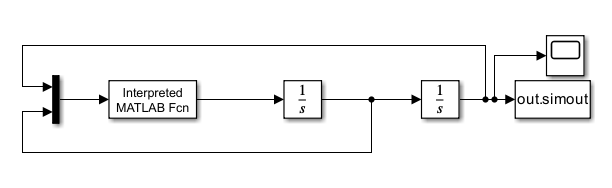
\includegraphics[width=0.49\textwidth]{imgs/5.png}
    \caption{Robot simulator using simulink}
    \label{fig:4.1}
\end{figure}

In the function "compute-q" we use the inputs (q,dq) to compute the gravity term, the Inertia matrix and the Coriolis matrix, and then we proceed to the calculations for the accelerations:

\begin{equation}
    \ddot{q} = M^{-1}(q) \times [\tau - g(q) - C(q,\dot{q})\dot{q}]
\end{equation}

where $\tau$ is only equal to the viscous friction term, because in these tests $\tau_c = 0$ and $\tau_e = 0$.

Now we have all the system built to run some tests. As mentioned in the statement we used different values for the  viscous friction term to see how it responds to it and to show this behaviour we created a function "showRobot.m" that is called several times to show the movement of the robot with the conditions given earlier.

\begin{figure}[H]
    \centering
    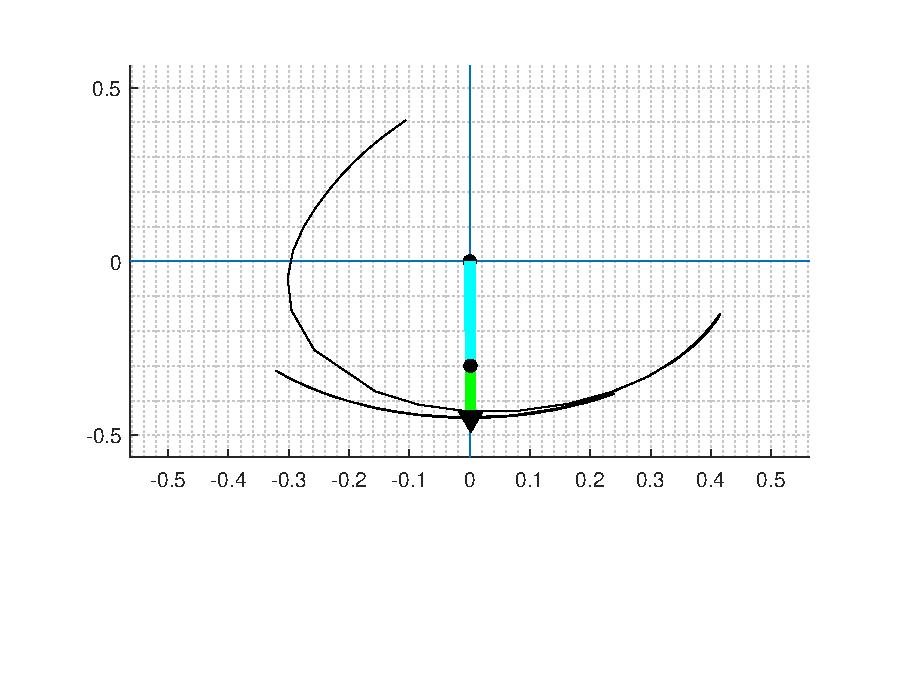
\includegraphics[width=0.49\textwidth]{imgs/4.1.eps}
    \caption{Robot simulator using simulink with Fv =0.05}
    \label{fig:4.2}
\end{figure}

\begin{figure}[H]
    \centering
    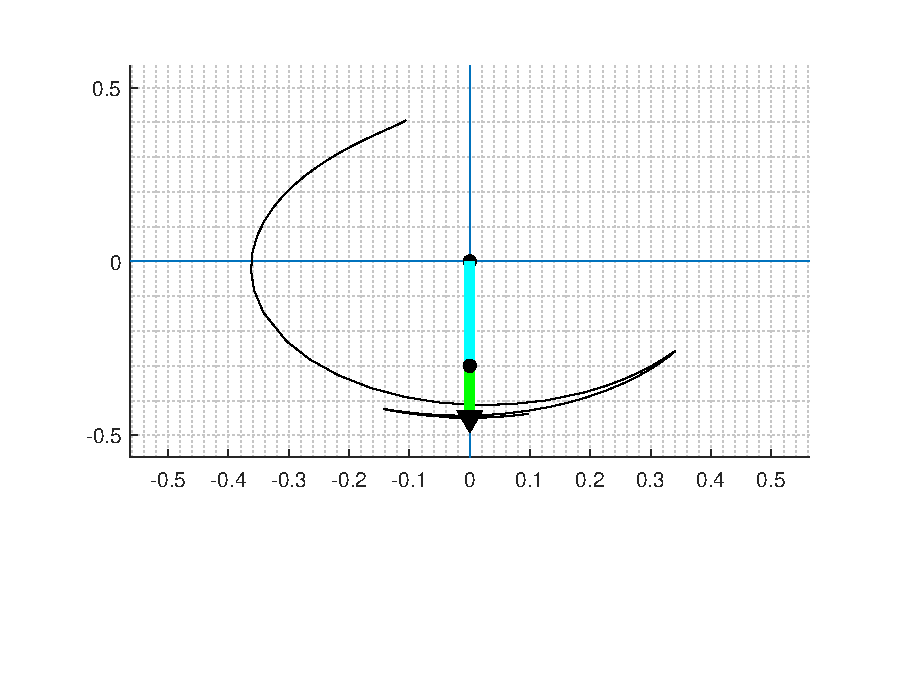
\includegraphics[width=0.49\textwidth]{imgs/4.2.eps}
    \caption{Robot simulator using simulink with Fv =0.1}
    \label{fig:4.3}
\end{figure}

\begin{figure}[H]
    \centering
    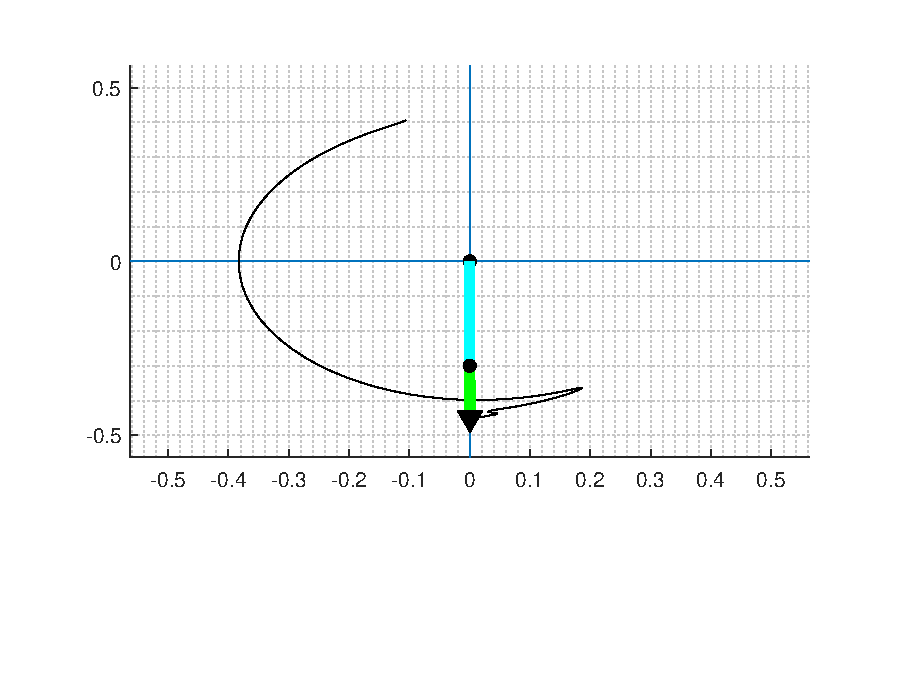
\includegraphics[width=0.49\textwidth]{imgs/4.3.eps}
    \caption{Robot simulator using simulink with Fv =0.2}
    \label{fig:4.4}
\end{figure}

\begin{figure}[H]
    \centering
    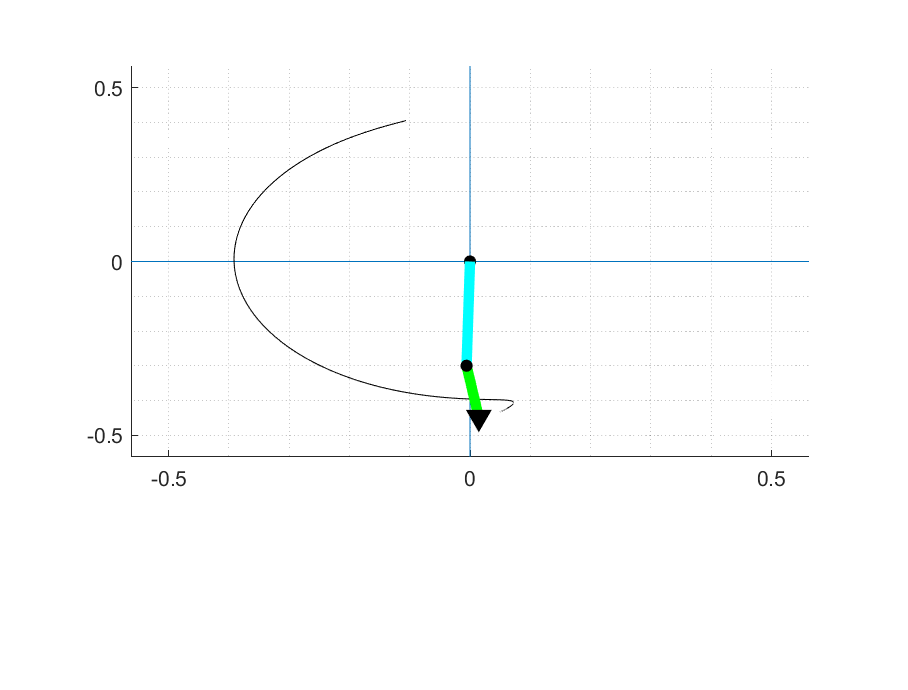
\includegraphics[width=0.49\textwidth]{imgs/4.4.eps}
    \caption{Robot simulator using simulink with Fv =0.5}
    \label{fig:4.5}
\end{figure}

Analysing the graphics we can see that the viscous friction term has some influence in the robot's behaviour. The higher this term is the slower is the move and it does not bounce to much in the bottom. So, it will need greater forces to vary its position, if we put an higher viscous friction term it won't move unless we provide higher forces. It can be seen in the images, but it can also be better visualized in the videos sent with the submission.

\subsection{5 - Tests with $\tau = g(q)$}

Now we are going to use gravity compensation and for that we define the torque, $\tau$, equal to the gravity term, $g(q)$ (this is the only change in the system comparing to the last one).

\begin{figure}[H]
    \centering
    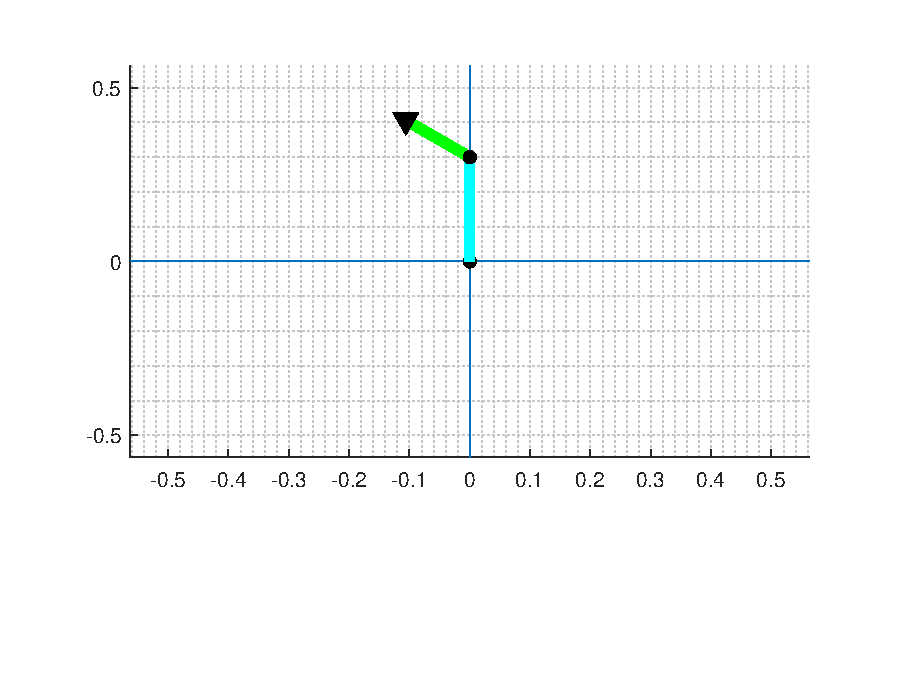
\includegraphics[width=0.49\textwidth]{imgs/5.1.eps}
    \caption{Robot simulator using simulink with $\tau = g(q)$}
    \label{fig:5}
\end{figure}

As expected the robot does not move as it can be seen in the  figure\eqref{fig:5} and in the vídeo, because the gravity is compensated and q1 and q2 don't vary.

\subsection{6 - Tests with different Cartesian forces}

Here we used different Cartesian forces applied to the robot’s end-effector and continued to use the gravity compensation. The forces are $F_c = [0 ,-10]^T$, $F_c = [10, 0]^T$ and $F_c = [10,-10]^T$.

To do these tests we just changed the torque expression as expressed in the notes given by professor in the theoretical classes.

\begin{equation}
    \tau = g(q) + J^TF_c
\end{equation}

This equation uses the Jacobian of the end-effector, J, calculated before, the cartesian forces applied and the gravity term, as it continues to be applied. Nothing else changes in the system, unless this equation

\begin{figure}[H]
    \centering
    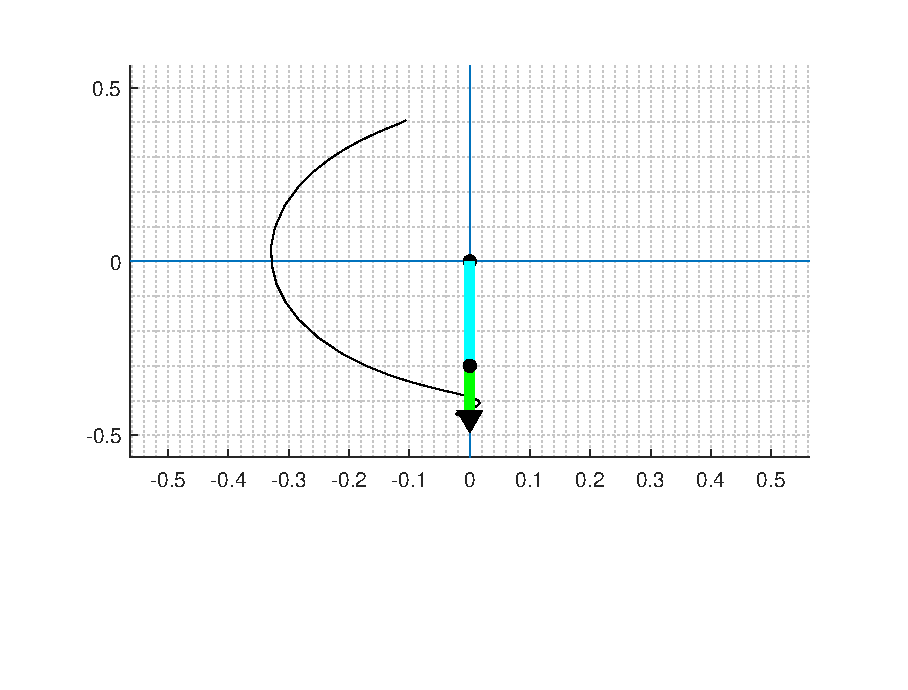
\includegraphics[width=0.49\textwidth]{imgs/6.1.eps}
    \caption{Robot simulator using simulink with $F_c = [0 ,-10]^T$}
    \label{fig:6.1}
\end{figure}

\begin{figure}[H]
    \centering
    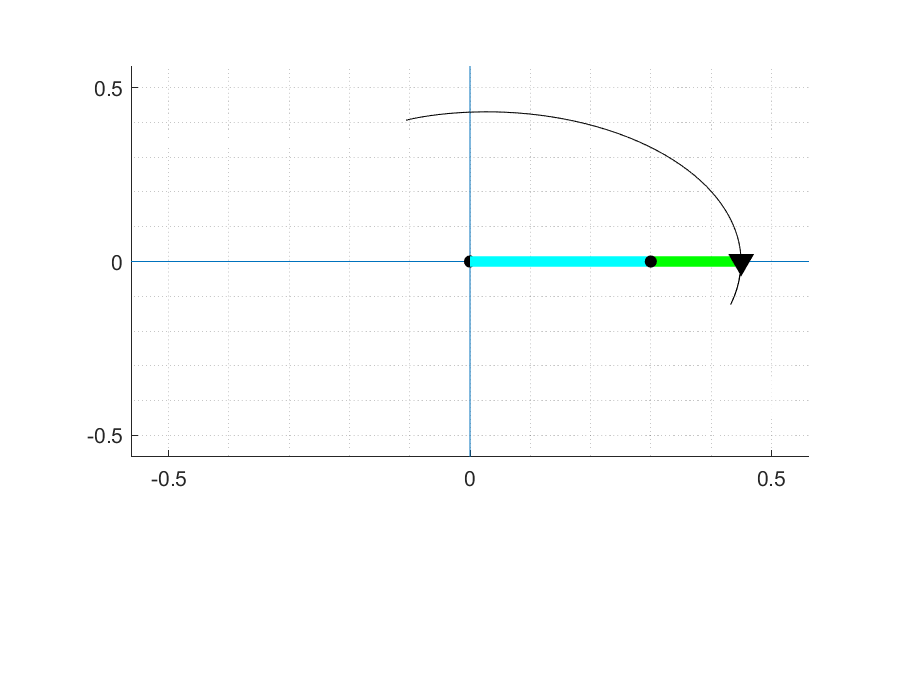
\includegraphics[width=0.49\textwidth]{imgs/6.2.eps}
    \caption{Robot simulator using simulink with $F_c = [10, 0]^T$}
    \label{fig:6.2}
\end{figure}

\begin{figure}[H]
    \centering
    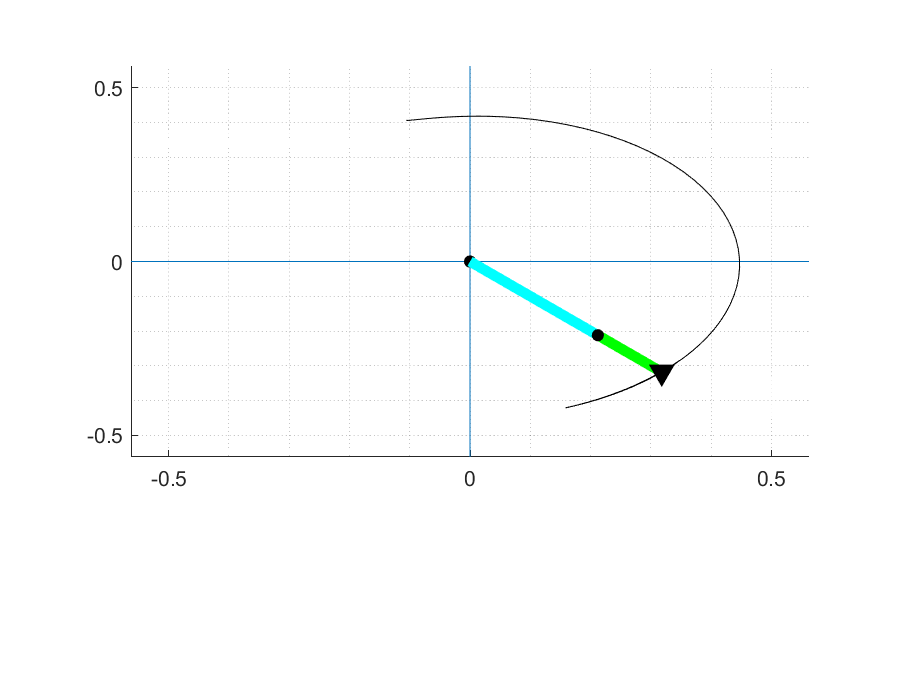
\includegraphics[width=0.49\textwidth]{imgs/6.3.eps}
    \caption{Robot simulator using simulink with $F_c = [10,-10]^T$ and $F_v = 0.5$}
    \label{fig:6.3}
\end{figure}

\begin{figure}[H]
    \centering
    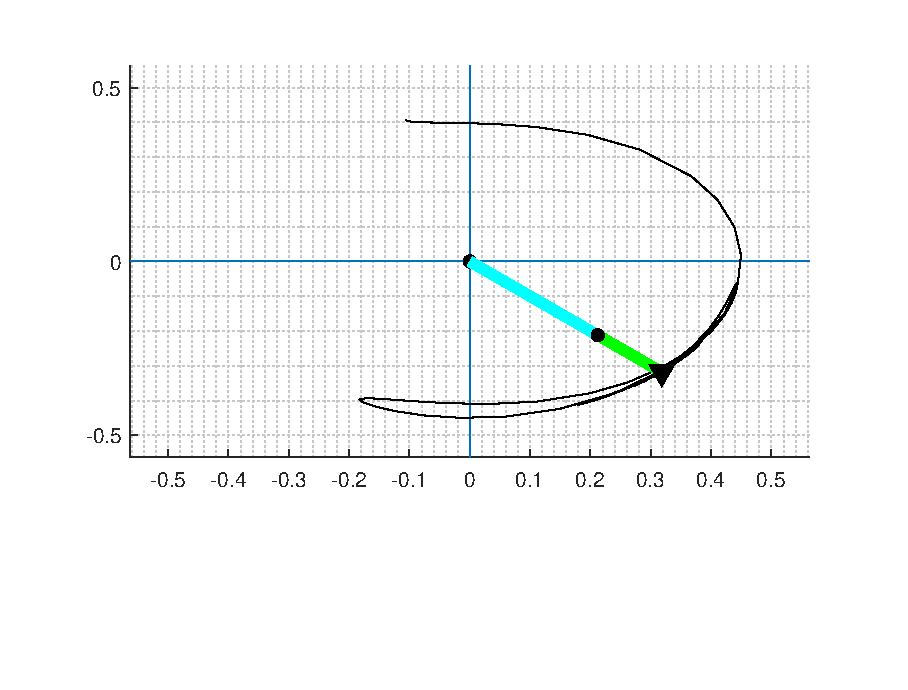
\includegraphics[width=0.49\textwidth]{imgs/6.4.eps}
    \caption{Robot simulator using simulink with $F_c = [10,-10]^T$ and $F_v = 0.1$}
    \label{fig:6.4}
\end{figure}



These figures\eqref{fig:6.1}\eqref{fig:6.2}\eqref{fig:6.3} are the results when using each one of the cartesian forces and the viscous friction term equal to 0.5, because was the last used. We can see that the end-effector goes to the position predicted, because of the use of cartesian forces. It is like the end effector is being pulled towards those directions. Another conclusion that we can get is that using a higher viscous term the behaviour is more smooth than using a lower viscous term, as we can compare in the figures\eqref{fig:6.3}, \eqref{fig:6.4} using a $F_v = 0.5$ and $F_v = 0.1$, respectively.

\subsection{7 - Tests for position control schemes in the task space}

There are two different methods to apply position control mentioned in the slides. Here we used the more basic approach, where a PID control is applied to the tracking error
of the robot, which is then converted to the joint space through the Jacobian matrix. We implemented these approach using the next simulink diagram.

\begin{figure}[H]
    \centering
    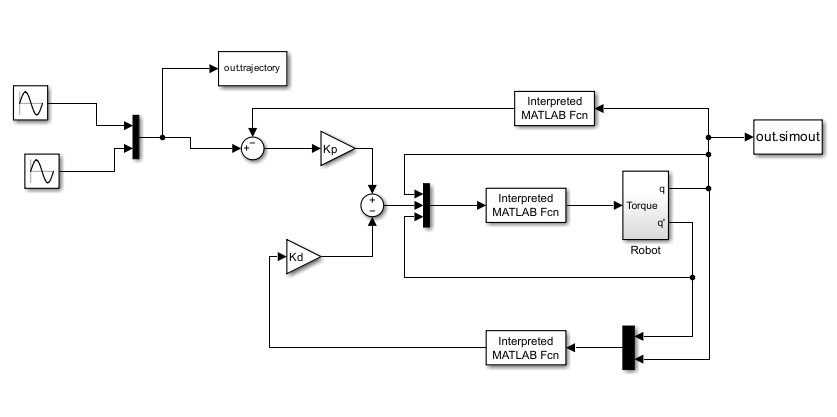
\includegraphics[width=0.49\textwidth]{imgs/7.1.png}
    \caption{Simulink for PD control}
    \label{fig:7.1}
\end{figure}

It can be seen in the figure \eqref{fig:7.1}, a PD control that is used to provide the position control. There we use functions like "X-7", "Xderivative-7" and "Dynamic-model-7" to make this control possible. This last function is where we implemented the basic approach for this control, and we only used P and PD control because is what is required for this part.

To test these control is said in the statement to generate an elliptical trajectory centered around (0.25, 0.2) with major axis $m_x = 0.12m$ and minor axis $m_y = 0.07m$ and to start with a cyclic frequency of 1/4 [Hz] with Simulink´s block "Sine Wave" on time based type.

To finally see the results we used PD control, but also, only a P control to see the differences, and tried to get some good values to his control. 

\begin{figure}[H]
    \centering
    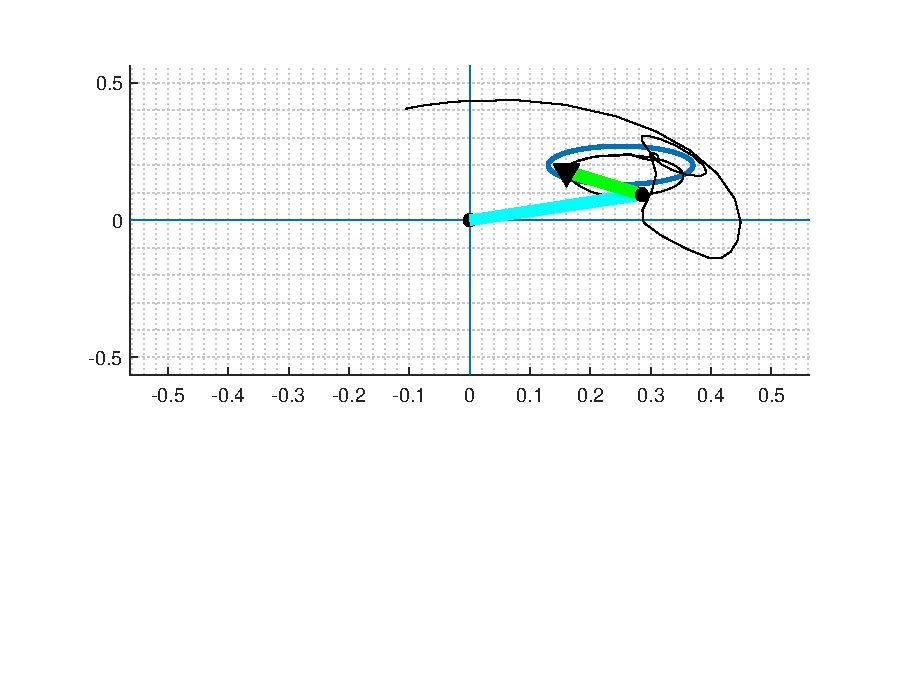
\includegraphics[width=0.49\textwidth]{imgs/7.2.eps}
    \caption{Robot simulator using simulink Kp=100}
    \label{fig:7.2}
\end{figure}

\begin{figure}[H]
    \centering
    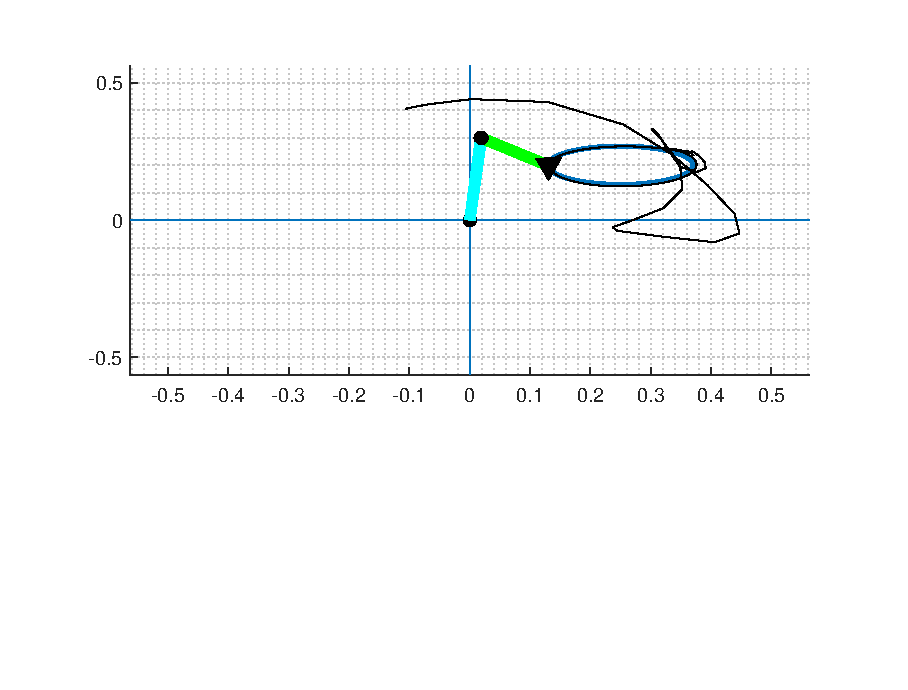
\includegraphics[width=0.49\textwidth]{imgs/7.3.eps}
    \caption{Robot simulator using simulink Kd=400}
    \label{fig:7.3}
\end{figure}

\begin{figure}[H]
    \centering
    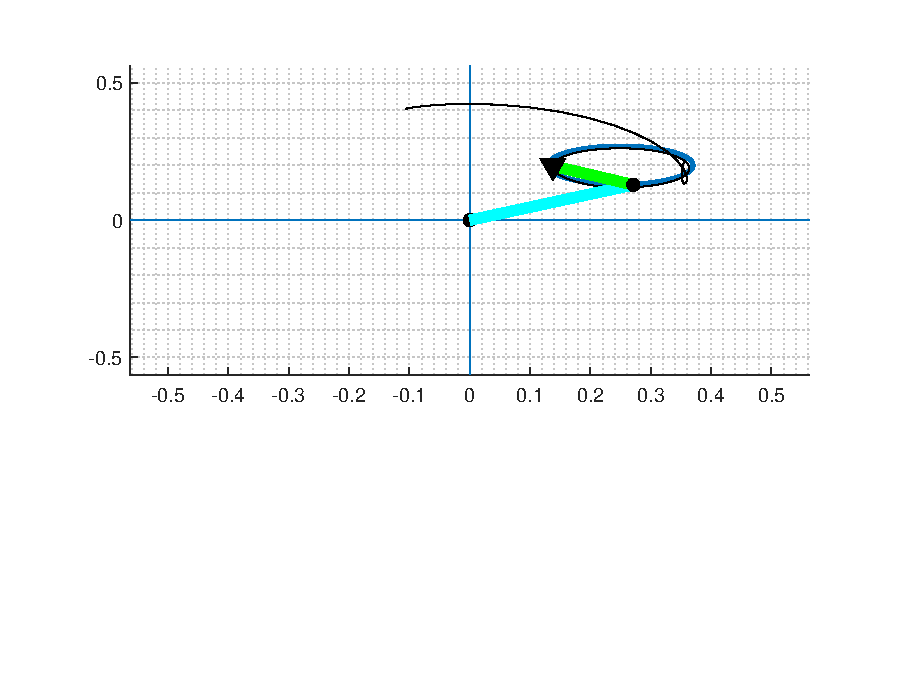
\includegraphics[width=0.49\textwidth]{imgs/7.4.eps}
    \caption{Robot simulator using simulink Kp=400 and Kd=10}
    \label{fig:7.4}
\end{figure}

\begin{figure}[H]
    \centering
    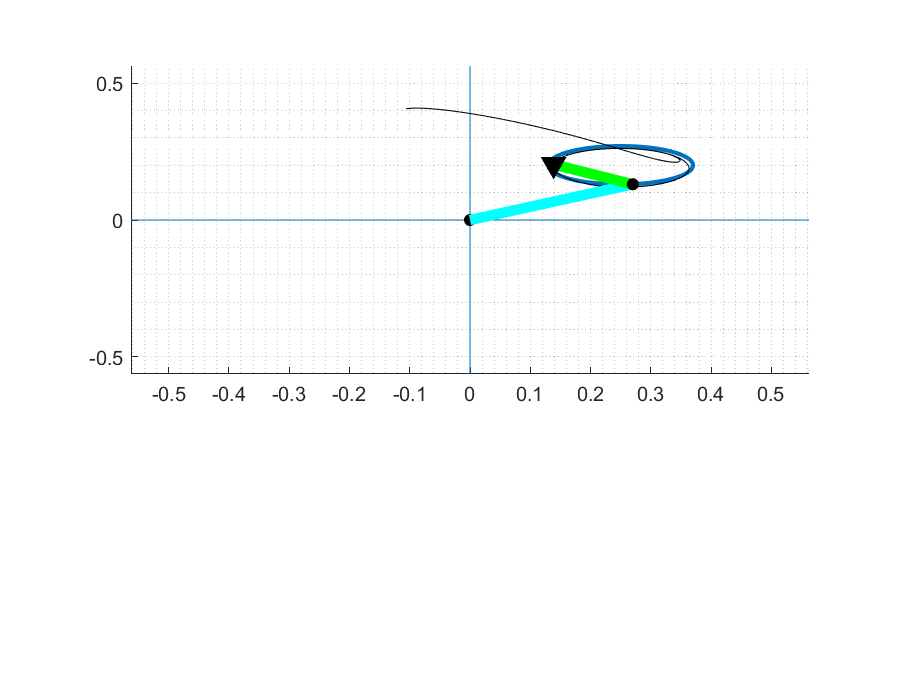
\includegraphics[width=0.49\textwidth]{imgs/7.5.eps}
    \caption{Robot simulator using simulink Kp=400 and Kd=30}
    \label{fig:7.5}
\end{figure}

Analysing the figures \eqref{fig:7.2}\eqref{fig:7.3} we can see that the position control is better using Kp=400, because the trajectory passes above the ellipsis while with Kp=100 the trajectory is a little outside the ellipsis. The steady-state tracking error is a little higher, but it is equal for the two of them, so concluding, with a Kp=400 we have a better performance.

Looking now for the figures \eqref{fig:7.4}\eqref{fig:7.5} we cannot see to many differences, the trajectory is full-filled but with Kd=30 the steady-state tracking error is small than using Kp=10, so the figure \eqref{fig:7.5} has a better performance.

Comparing now the P control with the PD control, we can say that the P control has worse response than the PD control, and the bigger difference is the minor steady-state tracking error.

It is also asked to make some tests with a vertical trajectory, for that we changed the parameter $m_x$ to 0 so that we can get a vertical line, and $m_y$ to 0.1 so we can get some thickness.

To test this control we used different values for the PD control (this time we used only PD control).

\begin{figure}[H]
    \centering
    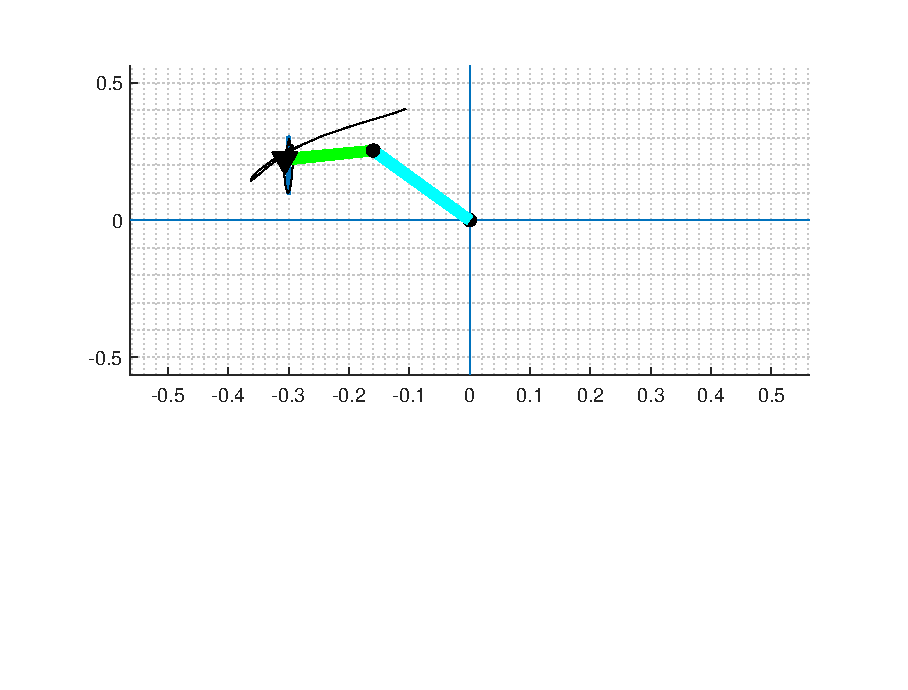
\includegraphics[width=0.49\textwidth]{imgs/71.1.eps}
    \caption{Robot simulator using simulink Kp=500 and Kd=10 in a vertical line}
    \label{fig:71.1}
\end{figure}

\begin{figure}[H]
    \centering
    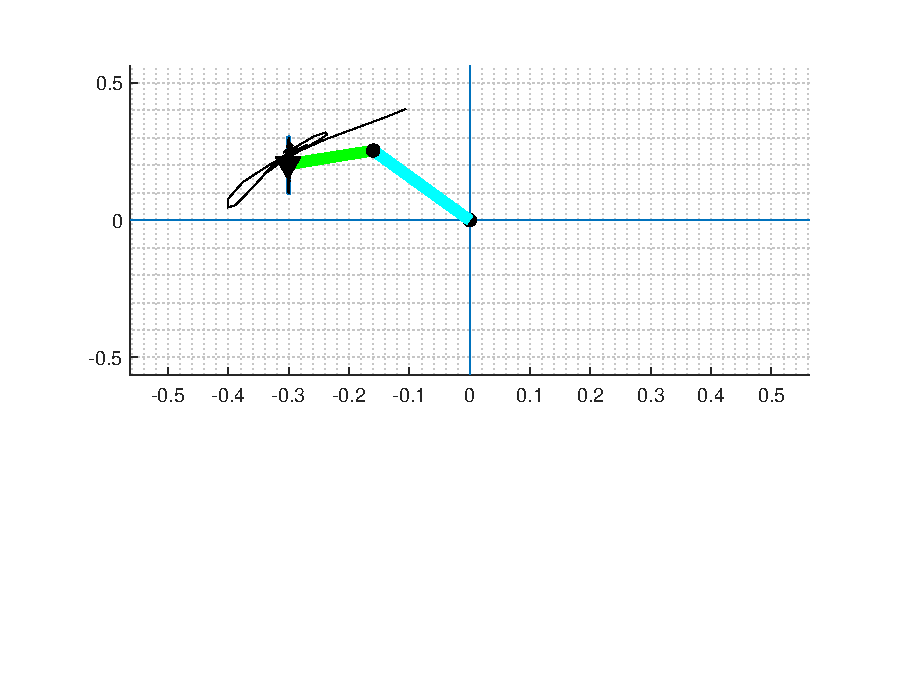
\includegraphics[width=0.49\textwidth]{imgs/71.2.eps}
    \caption{Robot simulator using simulink Kp=2800 and Kd=10 in a vertical line}
    \label{fig:71.2}
\end{figure}

\begin{figure}[H]
    \centering
    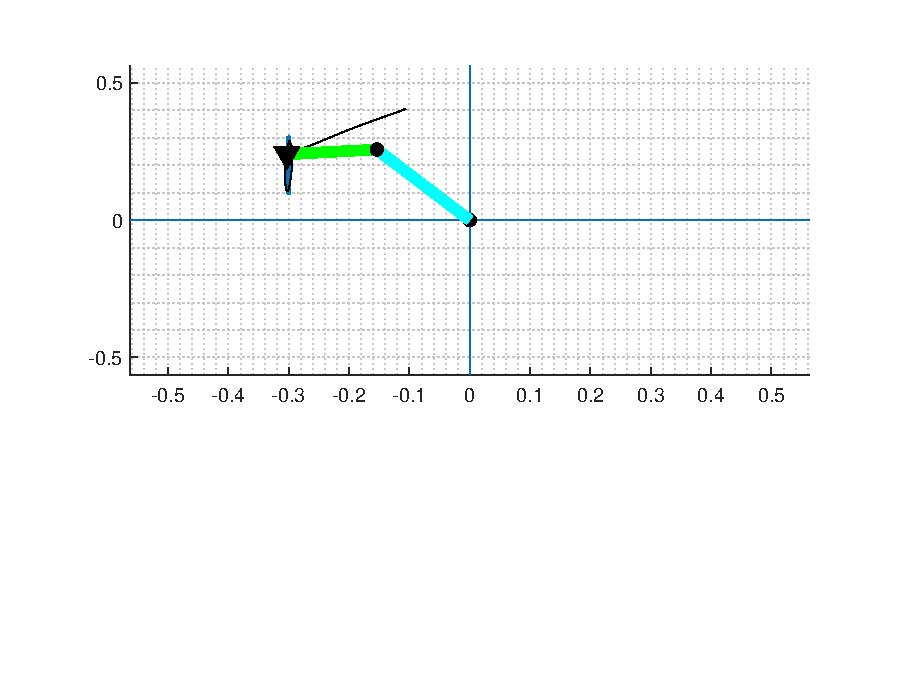
\includegraphics[width=0.49\textwidth]{imgs/71.3.eps}
    \caption{Robot simulator using simulink Kp=500 and Kd=90 in a vertical line}
    \label{fig:71.3}
\end{figure}

\begin{figure}[H]
    \centering
    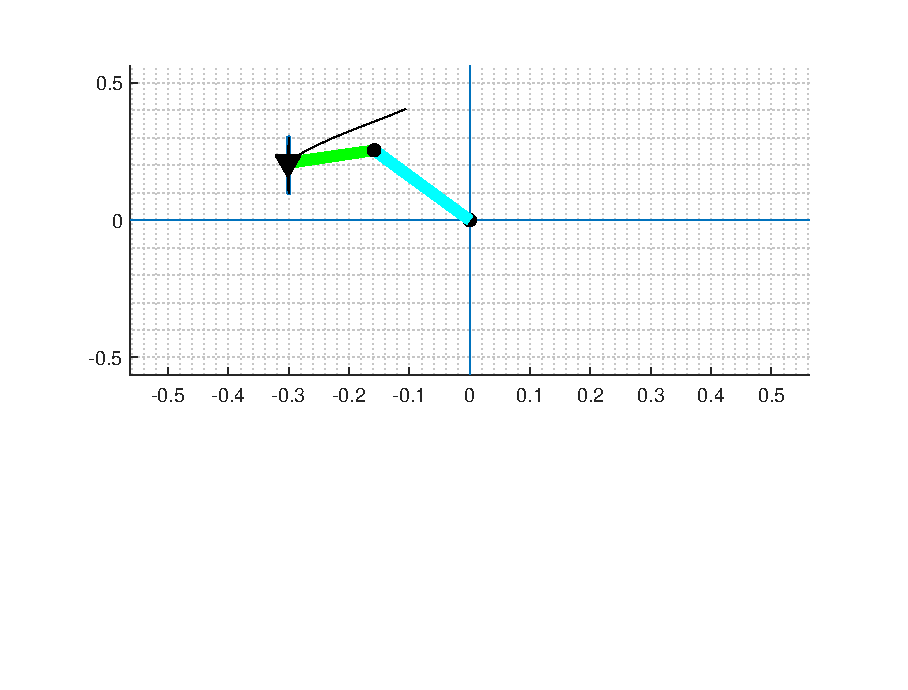
\includegraphics[width=0.49\textwidth]{imgs/71.4.eps}
    \caption{Robot simulator using simulink Kp=2800 and Kd=90 in a vertical line}
    \label{fig:71.4}
\end{figure}

Looking to the figures \eqref{fig:71.1} \eqref{fig:71.2} we can conclude that for the same Kd, a higher Kp makes the robot have a better trajectory over the vertical line but increases a little the steady-state tracking error. When we only change the parameter Kd the steady-state tracking error changes too and to decrease this error we use higher values for Kd like 90.

Finally we can conclude that the ideal parameters are Kp=2800 and Kd=90, where the performance is very good, the trajectory is over the vertical line, and there is not the steady-state tracking error. We also tried with higher values of Kp and Kd, but when increasing Kp higher than 2800, we start having some overshoot, and when we increase Kd for values over 90, the system turns to be more expensive computationally speaking, and the movement becomes slower too.

\subsection{8 - Tests for Compliance Control}

To implement the compliance control we first started by the data needed to the implementation and then we worked on the simulink so we could simulate the compliance control. First, $x_e=[0.25,0.2]$ (is the position of the virtual bone), $k_e=\begin{bmatrix}
2000 & 0\\
0 & 2000
\end{bmatrix}$, (is the stiffness of the bone), $k_p=2800$,$K_d=90$, and $Kp=\begin{bmatrix}
10000 & 0\\
0 & 10000
\end{bmatrix}$ (the values for the Pd control).

Now passing to the simulink, we did as the simulink used for the previous exercise figure\eqref{fig:7.1}, but we did some adaptations to the Function inside the simulink so we could use the external force applied to the robot that simulates an interaction from the surgeon, and the force applied by the virtual bone. The external force is applied with $F_c=[80;80]$ at a specific interval of time (between 4.5s and 5.5s). To see the effect of this forces applied to the robot we created a trajectory that passes through the bone (that is represented as a black circle) and the supposed it's that the robot does not pass past that point, that is the center of the black circle.

\begin{figure}[H]
    \centering
    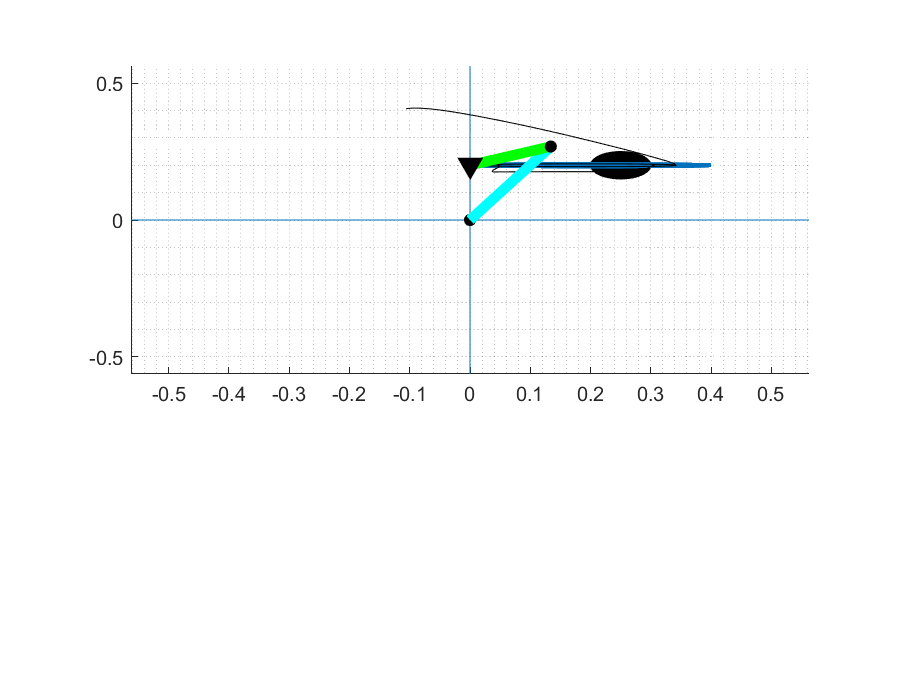
\includegraphics[width=0.49\textwidth]{imgs/8.1.eps}
    \caption{Robot simulator using simulink for Compliance control with the specific Ke}
    \label{fig:8.1}
\end{figure}

\begin{figure}[H]
    \centering
    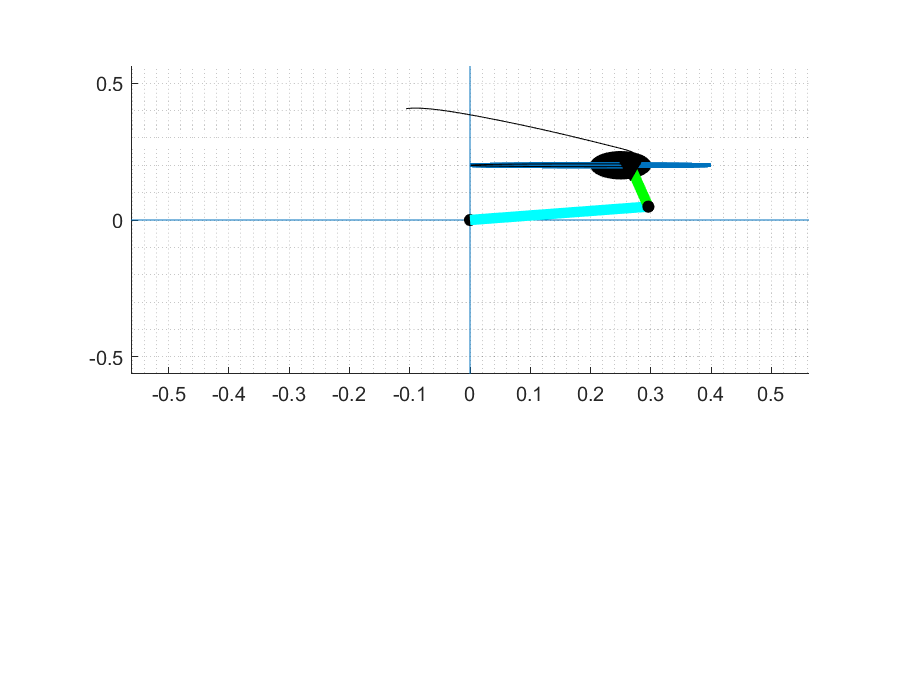
\includegraphics[width=0.49\textwidth]{imgs/8.2.eps}
    \caption{Robot simulator using simulink for Compliance control with a higher Ke}
    \label{fig:8.2}
\end{figure}

As results we have the figures \eqref{fig:8.1} \eqref{fig:8.2}, where in the first we used the supposed $K_e=2000$ and in the second we used a higher value, $K_e=20000000$ to see if it affected the robot. Analyzing the first one, the compliance control starts in the center of the black circle (virtual bone) and the robot decreases it's velocity, not completing it's trajectory, it could go a little more but the force doesn't let him. If the objective is to the robot to stop in the center of the virtual bone the $K_e$ needs to be higher, for that we used $K_e=20000000$ to see it's reaction. It can be seen in the figure and video that the robot when touches the center of the virtual bone, it decreases a lot it's velocity and stops after, not getting to the desired point, just like it's supposed. 

Talking now about the external force, the cartesian force, it can be seen, if we maximize that region, that we have a higher steady-state tracking error, that the robot does not fix because the control is only PD.

\subsection{9 - Tests for Impedance Control}

To implement the Impedance Control we started by the data needed and then we built the simulink. About the data we used the next values: $\dot{X}_D = [0;0]$ for the velocity and $\ddot{X}_D = [0;0]$ for the acceleration, a proportional gain $Pg = 1500$, a derivative gain $Dg = 40$, and the data for the impedance control: $K_d = \begin{bmatrix}
Pg & 0\\
0 & Pg
\end{bmatrix}$ , $D_d = \begin{bmatrix}
Dg & 0 \\
0 & Dg
\end{bmatrix}$, $M_d = \begin{bmatrix}
1 & 0\\
0 & 1
\end{bmatrix}$, $M_a = M_d/2$, $K_a = 0$ and $D_a = \begin{bmatrix}
0.5 & 0\\
0 & 0.5
\end{bmatrix}$.

Next we built the next simulink's block diagram with the matlab function "Dynamic-model-9" inside the block "Interpreted MATLAB Fcn".

\begin{figure}[H]
    \centering
    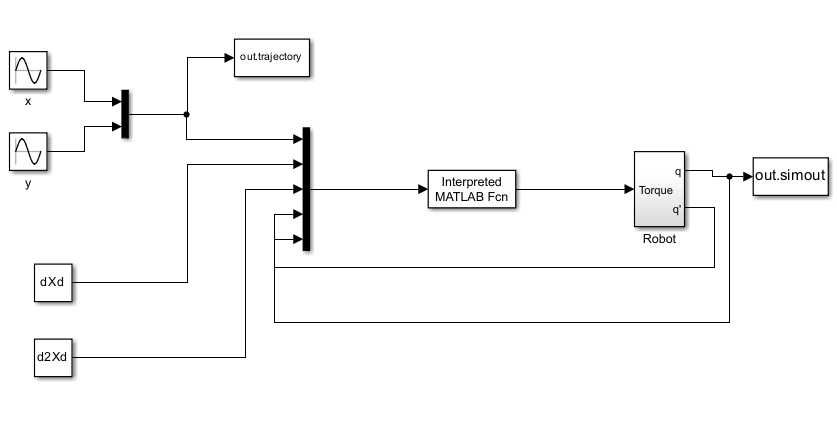
\includegraphics[width=0.49\textwidth]{imgs/9.1.png}
    \caption{Simulink for Impedance control}
    \label{fig:9.1}
\end{figure}

To observe if the behaviour of the robot is correct we applied a Cartesian force to the end-effector, equal to the one used before, in the compliance control, so that we can compare later, $F_c = [80;80]$, between 4.5s and 5.5s, therefore 1 second of external force applied.

\begin{figure}[H]
    \centering
    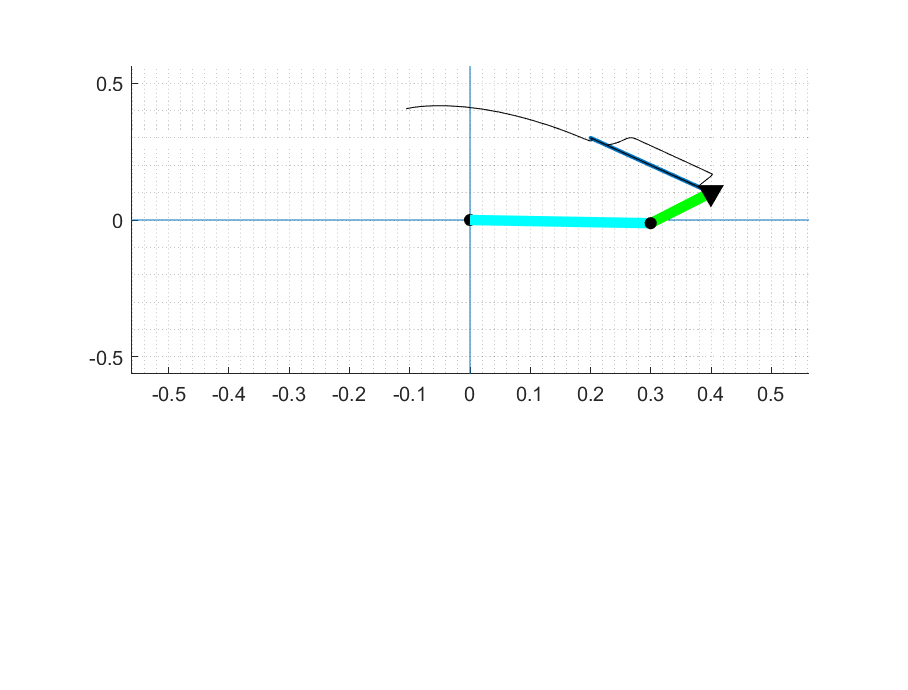
\includegraphics[width=0.49\textwidth]{imgs/9.2.eps}
    \caption{Robot simulator using simulink for Impedance Control}
    \label{fig:9.2}
\end{figure}

Analysing the figure \eqref{fig:9.2} we can see that the system has a good performance and it behaves as it is supposed. We tested for several different gains to see the best performance and we believe those values are good for the test, to decrease the overshoot and the steady-state tracking error.

We can now compare the Compliance control with the Impedance control. Looking to the figures \ref{fig:8.1},\ref{fig:9.2}, we can say that the compliance control could control better the external force, because the trajectory was closer to the one desired. These conclusion can only be make because it was used the same external force for both cases.




















